\documentclass{polytech/polytech}
\schooldepartment{di}
\typereport{custom}
\typereportname{Ajout PRD}
\reportyear{2017-2018}
\title{Plateforme d'acquisition et de formatage temps réel multiflux TV Web}
\student[di5]{Romain}{ROUSSEAU}{romain.rousseau@etu.univ-tours.fr}
\academicsupervisor[di]{Mathieu}{DELALANDRE}{mathieu.delalandre@univ-tours.fr}


\resume{Ce projet consiste en l'élaboration d'une plateforme d'acquisition de flux TV Web en temps réel. L'objectif dans un premier temps consistera en l'affichage de plusieurs flux en simultané avant d'éventuellement faire évoluer l'application pour y faire figurer des éléments d'analyse d'images. Au travers de ce rapport, nous verrons la démarche, les objectifs liés à la mise en place d'une telle plateforme, l'architecture logicielle avec une structure en multi-threads, ainsi qu'un état de l'art sur ce domaine constante expansion et qui représente près de 80\% du trafic de données sur Internet.}

\motcle{Plateforme d'acquisition} 
\motcle{Flux de données} 
\motcle{Temps réel}
\motcle{Protocole de communication} 
\motcle{Télévision en ligne}


\abstract{This project consists in the making of acquisition platform of Live TV streams in real time. The first aim is to display multiple streams at the same time before evolving the platform to add elements of frame analysis. Through this document, we will see the approach, the goals link in the making of such a platform, the software architecture with a multi-threaded structure, as a state-of-the-art in this constantly evolving domain which represents almost 80\% of data traffic on the Internet.}

\keyword{Streaming Platform}
\keyword{Live Stream}
\keyword{Real Time}
\keyword{Communication Protocol}
\keyword{Online TV}


\addbibresource{bibliographie.bib}

%%%%%%%%%%%%%%%%%%%%%%%%%%%%%%%%%%%%%%%%%%%%%%%%%%%%%%%%%%%%%%%%%%%%%%%%%%%%%%%%%%%%%%%%%%%%%%%%%%%
%%%%%%%%%%%%%%%%%%%%%%%%%%%%%%%%%%%%%%%%%%%%%%%%%%%%%%%%%%%%%%%%%%%%%%%%%%%%%%%%%%%%%%%%%%%%%%%%%%%

\begin{document}

\part{Test}


La télévision est diffusée dans le monde par divers moyens. Les plus traditionnels sont les suivants (CITATION Comment recevoir la télévision CSA)

\begin{description}
	\item[Diffusion hertzienne]: Elle consiste à diffuser les informations via le réseau hertzien en utilisant des antennes relais. La réception de ces données se fait grâce au antenne "râteau". En France, cette diffusion était sous forme analogique avant de passer en forme numérique avec la TNT (Télévision numérique terrestre). Il s'agit du type de réception le plus utilisé en France et qui possède une grande couverture du territoire (plus de 1600 antennes relais couvrant 97\% de la population métropolitaine).
	
	\item[Diffusion par satellite]: Cette méthode utilise des satellites en orbite géostationnaire pour retransmettre les chaînes de télévision. Une antenne parabolique est nécessaire pour recevoir les données. Ce principe couvre l'intégralité du territoire et permet ainsi de couvrir certaines zones d'ombre de système hertzien.

	\item[Diffusion par câble]: Ici les données sont diffusées via une réseau filaire spécifique. Ce principe est peu commun en ce France (dû à une couverture du territoire faible par ce réseau), mais il est le moyen le plus utilisé dans plusieurs pays occidentaux, notamment aux \'{E}tats-Unis.
	
	\item[Diffusion par internet]: Ce type de diffusion prend de plus en plus d'ampleur. Le principe réside dans la diffusion de donnée via Internet en général (venant d'une connexion ADSL, fibré, 4G, etc.). Le téléspectateur peut utiliser plusieurs moyens pour regarder les flux: avoir un boîtier récepteur fourni par un opérateur (exemple avec les différentes box et abonnements des fournisseurs d'accès à internet) ou bien en utilisant les flux disponibles sur des plateformes de visionnement en ligne (exemple avec les sites des chaînes de télévision qui proposent souvent de voir leur diffusion en direct).
	
\end{description}


Service par contournement, OTT service.
Les services OTT face aux moyens traditionnels 
D'où viennent les flux: natif, satellite, antenne...




%Fonctionnement de HTTP Dynamic streaming / Adobe Flash
%fichier f4f

An .F4F is a multimedia file fragment that is stored in the F4V flash video format. The F4F file contains a number of video file fragments that can be streamed through the HTTP dynamic streaming service and played back by the Flash video plug-in that is compatible with the F4V format. Further, the multiple video file fragments can be joined into a single video file for dynamically streaming the content. The F4F file is a proprietary file format that is compatible with Adobe Flash Player browser plug-in.


%Copyright et DRM

La technologie Digital Rights Management (DRM), soit en français la Gestion des droits numériques (GND), permet aux services multimédia en ligne de vérifier que le contenu qu'ils fournissent est utilisé correctement. Alors que certains contenus protégés par DRM peuvent être lus en utilisant les plugins Microsoft Silverlight ou Adobe Flash, beaucoup de services passent à la vidéo HTML5 qui requiert un système de DRM différent appelé Module de décryptage de contenu (CDM en anglais).



\chapter{Guide d'installation et d'utilisation}


\section{Pré-requis}


La plateforme est destinée à fonctionner sur les machines de l’école. Il est nécessaire d'avoir une configuration réseau et matérielle solide si l'on souhaite faire fonctionner un maximum de chaînes en simultané sur l'application. La configuration minimale requise est la suivante :

\begin{itemize}
	\item Windows 7 Pro 64 bits
	\item Intel Xen CPU 3.06GHz
	\item 2 processeurs
	\item 4 Go de RAM
\end{itemize}


Pour la configuration réseau, la plateforme peut fonctionner sur un réseau Wi-Fi domicile mais la charge plafonne autour de 7 streams de qualité moyenne.


\section{Installations}

L'application nécessite plusieurs installations:

\subsection{Streamlink}

Streamlink est le logiciel en Python qui va prendre en charge les streams et qui va activer les flux à lire. Il existe plusieurs moyens de se procurer \textit{streamlink}, le plus simple est l'exécutable disponible à l'adresse : https://github.com/streamlink/streamlink/releases .

L'application fonctionne pour les versions 0.10.0 et supérieurs.

\subsection{VLC}

VLC est le logiciel permettant à l'application de visualiser les chaînes. Le programme  fonctionne avec la version 3.0.1 de VLC disponible à l'adresse suivante : https://get.videolan.org/vlc/3.0.1/win64/vlc-3.0.1-win64.exe


\subsection{Java Runtime Environment}

Le programme est un fichier jar qui fonctionne sur la version 8 de Java. Il est nécessaire pour le faire fonctionner de disposer du JRE 8 disponible à l'adresse : www.oracle.com/technetwork/java/javase/downloads/jre8-downloads-2133155.html


\section{Récupération du projet et fonctionnement}

Le projet se trouve sur le dépôt GitHub disponible à l'adresse suivante : https://github.com/RomainR37/streamPlatform

Une fois sur cette page, vous pouvez soit cloner le dépôt Git sur votre ordinateur, soit télécharger le dossier compressé en cliquant sur le bouton \textit{Clone or download} puis en sélectionnant son choix.

Après avoir récupérer le projet, vous pouvez l'exécuter en lancer une invit de commande Windows (en tapant Win+R au clavier puis \textit{cmd} dans le champ disponible). Une fois sur l'invit, dirigez vous vers le dossier du projet récupéré puis dans le dossier, allez dans le dossier \textit{target}. Il contient le fichier jar exécutable et un fichier texte exemple \textit{testStream.txt}. Pour lancer l'application avec le fichier \textit{testStream.txt} à disposition, la commande est la suivante : \javacode{java -jar streamPlatform-1.0.0-jar-with-dependencies.jar testStream.txt}. L'application se lancera.

\begin{figure}
	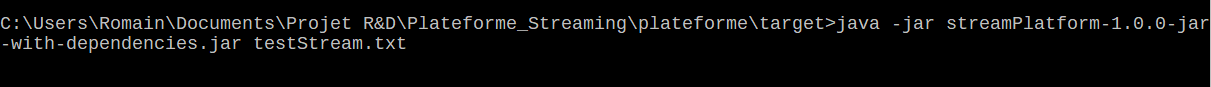
\includegraphics[scale=0.6]{images/cmdLancement.png}
	\caption{Commande de lancement du programme}
\end{figure}


\section{Fichier texte et syntaxe}

Il est possible de lancer l'application avec le fichier texte que l'on souhaite. Celui-ci pour fonctionner devra se situer dans le dossier \textit{target} également. Cependant le fichier doit respecter une convention de nommage. 


Une chaîne nécessite deux informations pour pouvoir fonctionner: son nom et l'adresse du site diffusant son stream. Dans le fichier texte que l'on veut lire, ces deux informations doivent transparaître séparées d'une tabulation. Vous pouvez voir l'exemple du fichier \textit{testStream.txt} ci-après:

\begin{figure}
	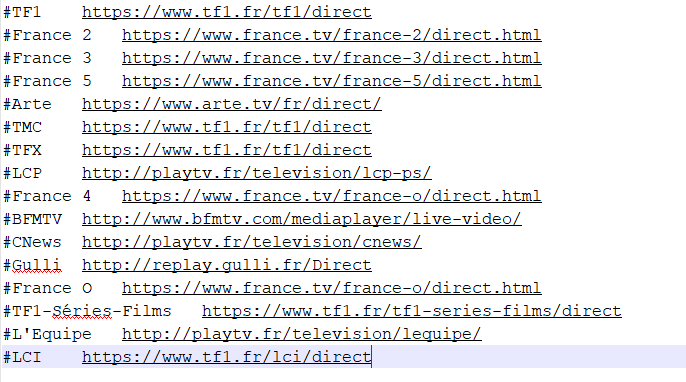
\includegraphics[scale=0.7]{images/testStream.png}
	\caption{Fichier texte exemple \textit{testStream}}
	\label{fig:fichier_texte}
\end{figure}

Ici sur la \autoref{fig:fichier_texte}, nous pouvons voir un \# avant une ligne. Il s'agit de la notation pour mettre une ligne en commentaire. Ainsi, le fichier \textit{testStream.txt} contient déjà une quinzaine de chaînes de télévision fonctionnelles, il suffit donc de supprimer les \# devant la chaîne que l'on veut visualiser. Néanmoins, il est possible de rajouter de nouvelles chaînes tant qu'elle respecte la convention. 

Certaines chaînes ne fonctionnent pas avec streamlink, et ne sont donc pas disponibles sur l'application. Par exemple, la version 0.11.0 de streamlink ne prend pas en charge les chaînes diffusées sur Dailymotion. Le problème sera sans doute réglé dans les prochaines versions ce qui rajoutera de nouvelles chaînes disponibles au visionnage. 


\section{Problèmes pouvant survenir}



\subsection{Pare-feu de Windows}

Un message du firewall peut apparaître au lancement de l'application. Cela est dû au script Python lancé par Streamlink. Il suffit que le firewall accepte les scripts pour que le fonctionnement se passe correctement. 


\subsection{Problèmes d'affichage}

Sur certaines machines, et en particulier sur les machines virtuelles de l'école, il est possible de constater des problèmes d'affichage des chaînes. On peut voir en effet sur des streams de bonne qualité, des problèmes au niveau des contours sur l'image (comme sur la \autoref{fig:pbAffichage}, en particulier à droite de l'image).


\begin{figure}
	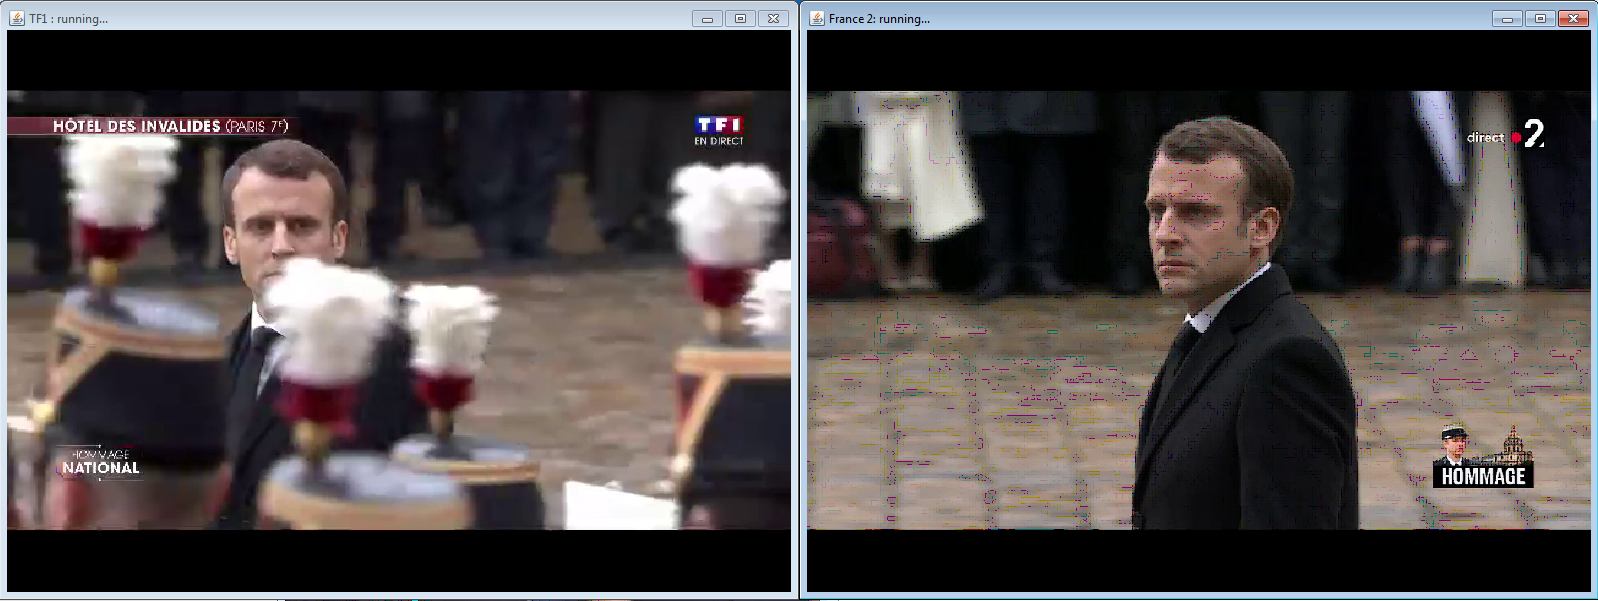
\includegraphics[scale=0.37]{images/imageQualite.png}
	\caption{Exemple de problèmes d'affichage}
	\label{fig:pbAffichage}
\end{figure}


Ces problèmes peuvent venir des configurations graphiques de la machine, notamment de DirectX. Néanmoins, lors des tests effectués sur machines Windows 10, il n'y avait aucun problème d'affichage, donc cela pourrait être des anciens systèmes Windows également.



\chapter{Utilisation de SonarQube}

Pour le développement du site, nous nous sommes servis de l'outil de qualité de code \textit{SonarQube}. C'est un logiciel libre permettant de mesurer la qualité du code produit en se basant sur divers règles mises en place au préalable. Il peut détecter les bugs potentiels, les duplications de code, la couverture de code par les tests unitaires, et bien d'autres. Il supporte plus de 25 langages et s'adapte aux outils de build traditionnels (Ant, Maven, Gradle) ainsi qu'à certains IDE comme Eclipse. Il est aussi adaptable et personnalisable selon les besoins avec de nombreux plug-ins à disposition.

L'installation de SonarQube se fait très simplement. Il suffit de télécharger le programme, puis de lancer le script StartSonar.bat. Une instance de SonarQube sera lancée, et une fois que le message "\textit{SonarQube is up}" s'incrit sur la console comme on peut le voir sur la \autoref{fig:sonarcmd}, nous pouvons ouvrir la page du programme sur un navigateur. Par défaut, SonarQube utilise le port 9000 sur l'hôte local.


\begin{figure}
	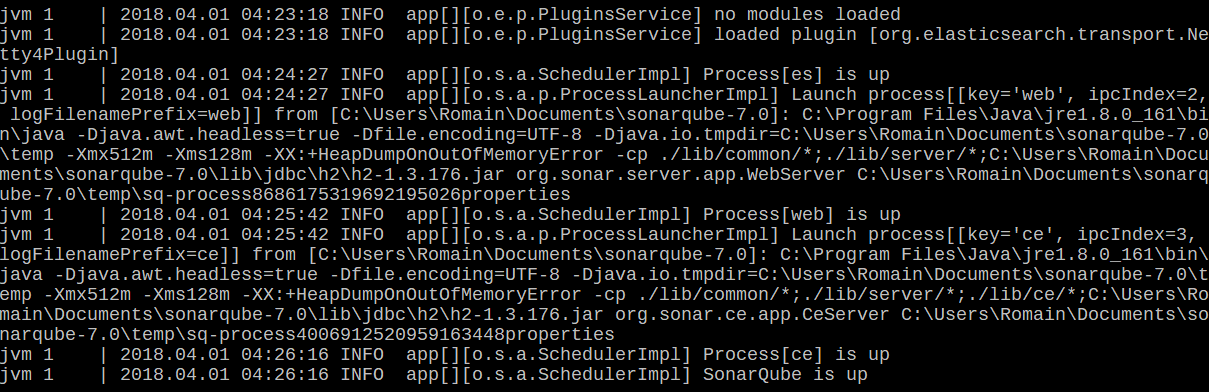
\includegraphics[scale=0.6]{sonarcmd.png}
	\caption{Lancement de l'instance SonarQube}
	\label{fig:sonarcmd}
\end{figure}


Maintenant que SonarQube est opérationnel, nous allons analyser notre projet. Dans un premier temps, nous regarderons l'application Angular. Dans notre cas, on souhaite que Sonar examine les fichiers \textit{typescript}. \'{E}tant donné que nous n'avons pas utilisé d'outils de build pour cette partie, nous avons installé un scanner sonar pour tout type de projet. Pour effectuer une analyse, il suffit de lancer depuis un terminal le script \textit{sonar-scanner} et de créer un fichier \textit{sonar-project.properties} comportant les détails concernant le projet, l'analyse s'effectuera par la suite. Le script va scanner tous les fichiers du dossier depuis lequel nous exécutons le programme et déterminera les éléments à modifier dans le code. Les résultats seront affichés dans l'instance SonarQube sur le navigateur internet.


Lors de notre première analyse sur l'application, nous avons eu les résultats suivants: 

\begin{figure}
	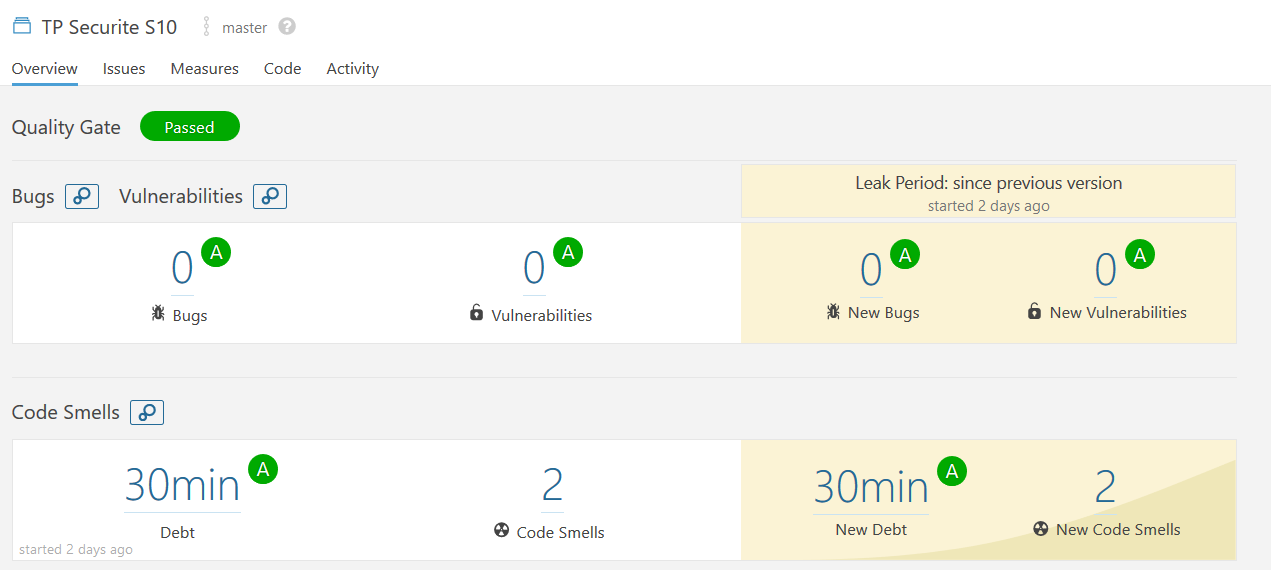
\includegraphics[scale=0.55]{sonarresult.png}
	\caption{Résultats de l'analyse Sonar}
	\label{fig:sonarresult}
\end{figure}

Nous pouvons remarquer que nous avons produit un code sans bug et sans vulnérabilités tout de suite, ce qui est déjà une très bonne chose. Il ne reste ainsi seulement qu'à corriger les deux erreurs détectées par Sonar pour avoir un code qui respecte les règles de Sonar. 


\chapter{Environnement de tests Angular}


Pour réaliser les tests unitaires de notre application, nous avons opté pour les frameworks de base recommandés par Angular, c'est-à-dire Karma et Jasmine. Karma est un runner de tests tandis que Jasmine est un reporter d'informations dans une fenêtre de navigateur. La configuration de ces deux outils se fait automatiquement par le gestionnaire Angular, mais il est possible de les adapter avec le fichier \textit{karma.conf.js} pour changer le port utilisé (par défaut il s'agit du 9876) ou encore de navigateur utilisé (par défaut, Karma utilise Chrome, pour l'utilisation d'un autre navigateur, il faut installer un plug-in particulier). L'une des grandes forces de ces outils est qu'ils ne nécessitent pas une compilation systématique pour avoir un visuel de la solution. Ici, chaque modification apportée aux tests est visible dans l'immédiat sur le navigateur. 

Les fichiers de tests d'Angular se distinguent par les extensions \textit{.spec.ts}. Ces fichiers sont analysés par Karma pour lancer les tests. Pour utiliser Karma, il suffit de lancer la commande \javacode{ng test}. Puis, à partir du navigateur, nous pouvons voir les tests s'exécuter en temps réel. 

\begin{figure}
	\includegraphics[scale=1]{karma.png}
	\caption{Lancement de Karma}
	\label{fig:karma}
\end{figure}

Dans la \autoref{fig:karma}, on peut voir que nos premières spécifications ont échoué. Elles sont dues à un module qui a été mal importé. Une fois corrigé, les tests passaient sans problème.

Les tests que nous avons réalisés concernent principalement l'affichage et le rendu général de l'application, avec des vérifications sur le titre du site, sur la présence de certaines balises à l'affichage, etc. Il aurait été intéressant de tester les liaisons entre l'appli Angular et la partie Symfony avec des outils comme Mockito par exemple, mais cela nous aurait nécessité plus de temps. 

\end{document}